\section{Problem formulation}
\label{sec:problem}

We formalize the co-evolution of construction principles and learner capabilities, with curriculum allocation modeled as a sequential decision problem. At round $e$, capability-specific shares $\boldsymbol q_e$ allocate a finite construction budget across capability cells defined within each task, subject to fixed task-level quotas. Construction principles $\Sigma_e$ are reusable specifications that determine how medical evidence is organized into supervision for a target capability. These principles define question intent, guide how responses draw on medical evidence, and clarify conceptual distinctions.

\subsection{Learner state and curriculum allocation}

At round $e$, the learner $M_e$ is assessed on independent validation sets $\mathcal V=\{\mathcal V_t\}_{t\in\mathcal T}$ for tasks $\mathcal T$. Support set $\mathcal S$ supplies medical visual evidence and associated text for supervision construction; independent external benchmarks evaluate generalization. Predefined capability cells form $\mathcal C$, with each cell $c$ assessed on a fixed nonempty subset $\mathcal V_c\subseteq\mathcal V_t$. A capability evaluation functional $\mathcal J_c$ maps predictive behavior to empirical mastery:
\begin{equation}
\mathcal J_c[M_e]=\frac{1}{|\mathcal V_c|}\sum_{z\in\mathcal V_c}u_c(M_e,z),
\qquad
\widehat{\boldsymbol\kappa}_e=\bigl(\mathcal J_c[M_e]\bigr)_{c\in\mathcal C}.
\label{eq:capability_level}
\end{equation}
Here $u_c$ is a fixed evaluation rule that assigns a score to each example, with higher scores indicating better performance. The vector $\widehat{\boldsymbol\kappa}_e$ is the observable capability profile. Task performance and error evidence constitute observation $o_e$.

The curriculum planner selects action $a_e$ from history summary $\mathbf{s}_e=\Phi(h_e)$, where $h_e$ records observations, actions, and rewards through round $e$. We model this interaction as a finite-horizon partially observable Markov decision process~\citep{kaelbling1998planning,matiisen2017teacher}. The complete state $X_e$ includes learner parameters and optimization state, active construction principles, revision history, scheduling information, and remaining resources. Under the rule $\mathscr E$ governing principle evolution,
\begin{equation}
P(X_{e+1}\mid X_{0:e},a_{0:e})
=P_{\mathscr E}(X_{e+1}\mid X_e,a_e).
\label{eq:transition}
\end{equation}
The transition comprises supervision construction, verification, learner updates, and principle revision driven by learning responses. Appendix~\ref{app:formalization} specifies the state and observation model.

% Queue the full-width framework for the next page top before the method section.
\begin{figure}[!t]
\centering
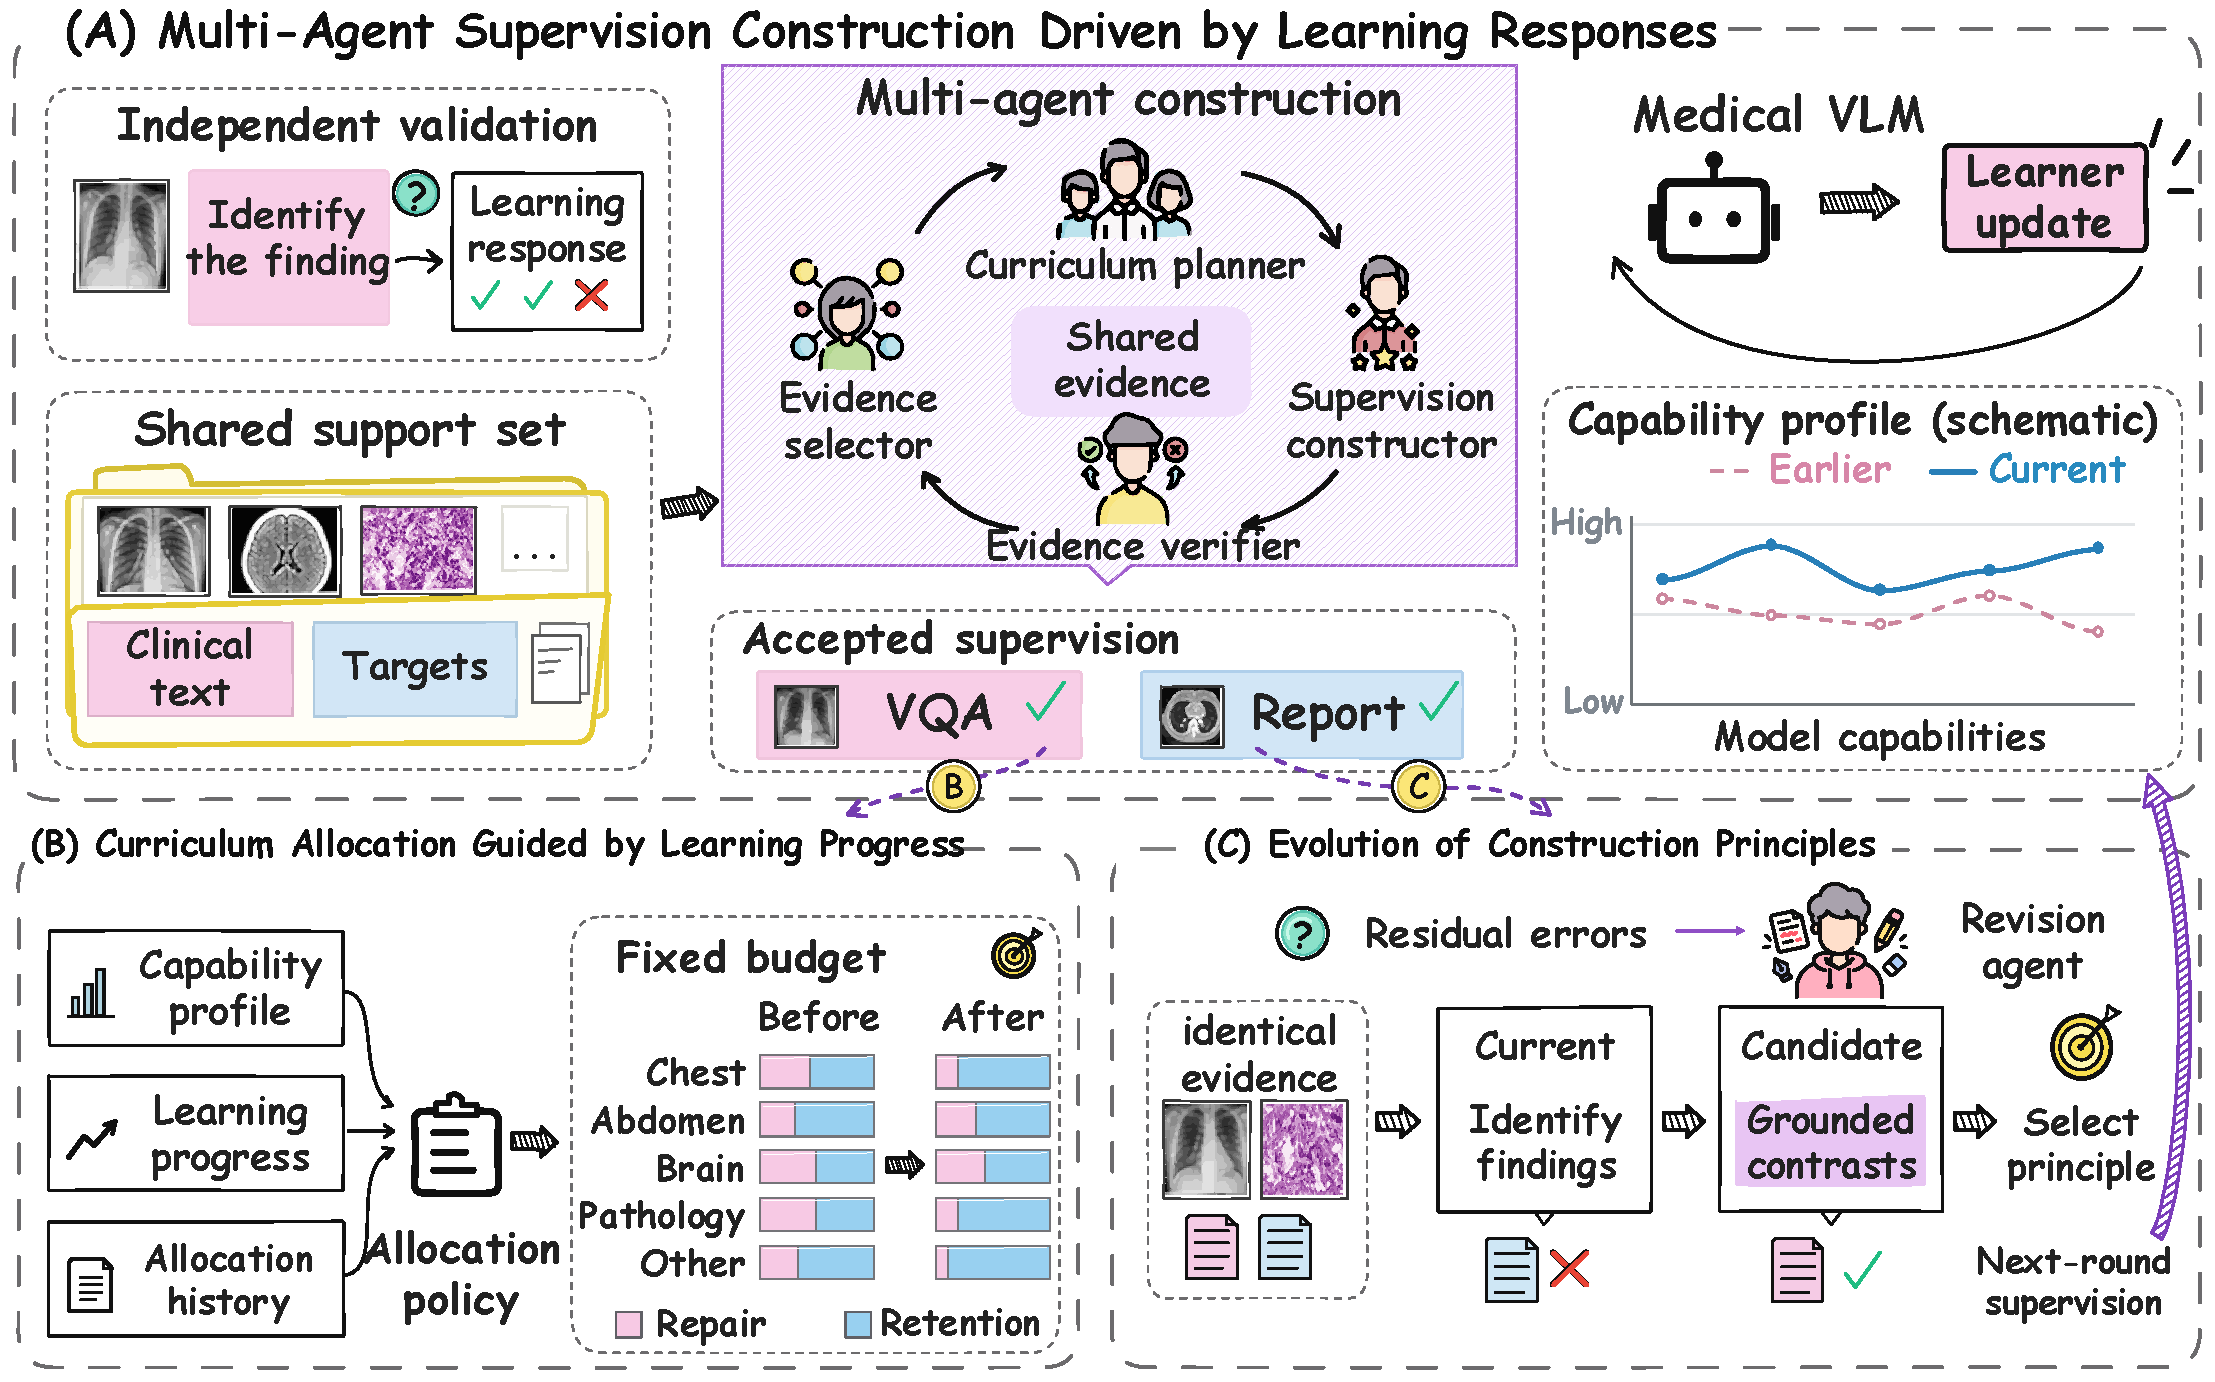
\includegraphics[width=\linewidth]{figures/evoforma_framework.pdf}
\caption{CoEvoMed framework. (A) Multi-agent collaboration constructs and verifies supervision from medical evidence; learner updates yield responses on independent task validation sets. (B) Learning progress guides curriculum allocation under fixed task budgets. (C) The revision agent uses learner responses to revise construction principles and compares supervision generated by current and candidate principles from the same evidence; accepted revisions guide subsequent construction.}
\label{fig:framework}
\end{figure}


\subsection{Supervision construction}
\label{sec:supervision_evolution}

Candidate training examples $z=(v,x,y)$ comprise a visual input, instruction, and target response, with distribution
\begin{equation}
\widetilde p_e(z)=\sum_{c\in\mathcal C}q_{e,c}\,
g_{e,c}(z;\Sigma_e,\mathcal S).
\label{eq:supervision_mixture}
\end{equation}
Here $g_{e,c}$ denotes the probability distribution over candidate training examples for capability cell $c$ at round $e$, induced by evidence selection and supervision construction under $\Sigma_e$ using $\mathcal S$, before verification. Nonnegative shares $q_{e,c}$ sum to one. Principle evolution changes the component content, while allocation changes its relative investment. Evidence-grounded verification yields accepted supervision $\mathcal D_e^{\mathrm{syn}}$; subsequent mixing determines training exposure.

\subsection{Learner updates and policy objective}

The training mixture $\mathcal D_e^{\mathrm{mix}}$ combines accepted supervision $\mathcal D_e^{\mathrm{syn}}$ with permitted original or replay data $\mathcal R_e$ reserved for training. The learner update is
\begin{equation}
M_{e+1}=\mathcal U(M_e,\mathcal D_e^{\mathrm{mix}}),
\label{eq:learning_dynamics}
\end{equation}
where $\mathcal U$ follows the prescribed training procedure and optimization state. Successive capability profiles track the learner's development over $E$ rounds. Responses from $M_{e+1}$ enter $h_{e+1}$ and revise $\Sigma_{e+1}$ through Equation~\ref{eq:strategy_evolution}, linking principle evolution to subsequent learning.

Within these dynamics, the allocation policy maximizes cumulative validation progress:
\begin{equation}
\max_{\pi\in\Pi_{\mathrm{adm}}}
\E_{\pi}\left[\sum_{e=0}^{E-1}\gamma^e r_e\right],
\label{eq:objective}
\end{equation}
where $\Pi_{\mathrm{adm}}$ contains policies satisfying the construction budget and task quotas, and $\gamma\in[0,1]$ is the discount factor. The reward $r_e$ weights validation gains for VQA and report generation equally (Section~\ref{sec:curriculum}). Appendix~\ref{app:cumulative_gains} relates cumulative gains to performance across rounds.

\FloatBarrier

\section{CoEvoMed: co-evolving supervision agents and multimodal learners}
\label{sec:method}

CoEvoMed couples supervision construction with learner updates through learning responses (Figure~\ref{fig:framework}). Its multi-agent system integrates curriculum allocation and principle evolution: allocation directs construction effort, while revised principles change how the agents organize medical evidence into supervision.

\subsection{Multi-Agent Supervision Construction Driven by Learning Responses}
\label{sec:multiagent}

The curriculum planner translates capability feedback into allocation shares and construction targets. The evidence selector retrieves compatible visual records and supported facts from $\mathcal S$; the supervision constructor applies $\Sigma_e$ to form question--answer pairs or reports, and the evidence verifier checks factual consistency, visual dependence, validity, and duplication. Accepted supervision $\mathcal D_e^{\mathrm{syn}}$ retains evidence and principle provenance for subsequent assessment.

The learner minimizes negative log-likelihood over response tokens in $\mathcal D_e^{\mathrm{mix}}$ under the prescribed budget (Appendix~\ref{app:learner_objective}). After each update, CoEvoMed aligns successive predictions on the same task-validation cases. The observed increment for cell $c$ is
\begin{equation}
\widehat{\Delta\kappa}_e(c)=\mathcal J_c[M_e]-\mathcal J_c[M_{e-1}],
\quad e\geq1.
\label{eq:capability_change}
\end{equation}
Paired changes distinguish resolved deficiencies, regressions in acquired capabilities, and persistent gaps, identifying repair and retention needs beyond net progress. The summary $\mathbf{s}_e$ combines current mastery, these changes, and allocation history to guide curriculum allocation. Residual errors in the learner's responses reveal task-specific gaps between current capabilities and task demands; their semantics guide construction targets and principle revision.

An evolution window groups training rounds for assessing principle usage and learning responses. At each window's end, the revision agent proposes candidates from residual errors. Comparisons under matched evidence determine which revisions guide subsequent supervision construction (Section~\ref{sec:strategy_evolution}). The complete procedure appears in Appendix~\ref{app:algorithm}.

\subsection{Curriculum Allocation Guided by Learning Progress}
\label{sec:curriculum}

The curriculum planner uses the curriculum allocation policy to select $a_e\sim\mu_{\theta_e}(\cdot\mid \mathbf{s}_e)$, balancing repair and retention and deciding whether to focus on capabilities with the strongest error evidence. Repair targets unresolved gaps in weaker capabilities and recent regressions; retention maintains coverage of acquired capabilities. The allocation map $\mathcal A$ translates the action and historical evidence into construction shares:
\begin{equation}
\boldsymbol q_e=\mathcal A(a_e,h_e),\qquad
\sum_{c\in\mathcal C_t}q_{e,c}=\bar q_t,
\label{eq:quota}
\end{equation}
where $\mathcal C_t$ contains the cells of task $t$ and $\bar q_t$ is its prescribed share. Thus, adaptation redistributes investment within fixed task budgets. These shares weight candidates in Equation~\ref{eq:supervision_mixture}; verification and mixing determine realized training exposure.

Let $U_t^{\mathrm{val}}$ evaluate the learner on $\mathcal V_t$ and $\delta_{e,t}=U_t^{\mathrm{val}}(M_{e+1})-U_t^{\mathrm{val}}(M_e)$. The reward balances VQA tasks $\mathcal T_{\mathrm V}$ and report tasks $\mathcal T_{\mathrm R}$:
\begin{equation}
r_e=G_e=\frac{1}{2|\mathcal T_{\mathrm V}|}\sum_{t\in\mathcal T_{\mathrm V}}\delta_{e,t}
+\frac{1}{2|\mathcal T_{\mathrm R}|}\sum_{t\in\mathcal T_{\mathrm R}}\delta_{e,t}.
\label{eq:gain}
\end{equation}
Evaluation scales remain fixed, so the signed reward retains gains and regressions. Behavior cloning initializes the curriculum planner. PPO with generalized advantage estimation then optimizes Equation~\ref{eq:objective} through on-policy interactions with the learner~\citep{schulman2017proximal,schulman2016high}. Appendix~\ref{app:implementation} specifies the mixed policy and optimization settings.

% Queue Table 1 early to preserve its page-top placement.
\begin{table}[!t]
\centering\small
\caption{Medical VQA accuracy (\%). Bold marks CoEvoMed; its 8B scores use R7.}
\label{tab:main}
\setlength{\tabcolsep}{4pt}
\renewcommand{\arraystretch}{1.05}
\begin{tabularx}{\linewidth}{@{}Y*{4}{>{\centering\arraybackslash}p{0.14\linewidth}}@{}}
\toprule
Models & PMC-VQA & VQA-RAD & SLAKE & PathVQA\\
\MainResultsRows
\end{tabularx}
\end{table}

\subsection{Evolution of Construction Principles}
\label{sec:strategy_evolution}

Curriculum allocation controls construction effort across capabilities. Construction principles $\Sigma_e$ specify question intent, evidence--response relations, and conceptual distinctions; their suitability depends on the learner's capability state. CoEvoMed revises these reusable principles as learning needs evolve.

At each window's end, sufficiently used principles with nonpositive net repair are considered for revision, where net repair counts repaired cases minus regressed cases. The semantics of residual errors guide principle revision while the target capability and medical facts remain fixed. For example, localization errors motivate more explicit associations between regional evidence and the target response.

Current and candidate principles generate supervision from identical evidence under matched quotas. Selection assesses factual consistency and task alignment, including whether revisions express the targeted evidence associations, conceptual contrasts, or fact coverage. Usable yield (the proportion of evidence assignments producing usable supervision) and paired coverage (the proportion producing usable supervision under both principles) provide screening criteria; Appendix~\ref{app:implementation} specifies their thresholds.

Accepted revisions persist as active construction principles~\citep{zhang2026agentic}. Their supervision shapes learner updates, whose validation responses guide further revision:
\begin{equation}
\Sigma_{e+1}=\mathscr E(\Sigma_e,h_{e+1},\mathcal S).
\label{eq:strategy_evolution}
\end{equation}
Here $h_{e+1}$ includes observations and rewards after the learner update. The operator retains active principles between evolution boundaries and when candidates are rejected.

\section{Experiments}
\label{sec:experiments}

\subsection{Experimental setup}

The 2D suite comprises VQA-RAD, SLAKE, PMC-VQA, and PathVQA~\citep{lau2018dataset,liu2021slake,zhang2024pmc,he2020pathvqa}, plus MIMIC-CXR and IU-Xray report generation~\citep{johnson2019mimic,demnerfushman2016preparing}. 3D evaluation covers closed-ended M3D-VQA, open-ended 3D-RAD, and AMOS-MM reports~\citep{bai2024m3d,gai2025threedrad,ji2024amosmm}. Qwen3-VL-8B-Instruct~\citep{bai2025qwen3} is the primary learner; Gemma-3-4B-IT~\citep{gemmateam2025gemma} and InternVL3-9B~\citep{zhu2025internvl3} test cross-backbone applicability, with InternVL results in Appendix~\ref{app:internvl}. Task validation guides adaptation, support evidence grounds supervision, and external benchmarks measure outcomes. Published baselines include Hulu-Med~\citep{jiang2025hulumed}, Lingshu~\citep{lasateam2025lingshu}, MedVLSynther-7B~\citep{huang2026synthesizing}, and CURE-4B~\citep{messina2026cure}.



\subsection{Medical multimodal performance}

CoEvoMed-8B exceeds Hulu-Med-7B by 1.15--4.80 accuracy points across the four VQA benchmarks, while CoEvoMed-32B leads all compared models on each benchmark (Table~\ref{tab:main}). Report generation reaches 68.22 on IU-Xray at 8B and 64.33 on MIMIC-CXR at 32B (Figure~\ref{fig:report_results}). All six 8B results use R7, selected for the best overall cross-task balance.

From the same Qwen3-VL-8B initialization, CoEvoMed outperforms direct training on approximately 700,000 raw examples across all four VQA benchmarks while using fewer training examples (Appendix~\ref{app:raw_source}). This comparison supports adaptive supervision construction and curriculum allocation as a source of performance gains beyond the volume of raw data.



\begin{figure}[!htb]
\centering
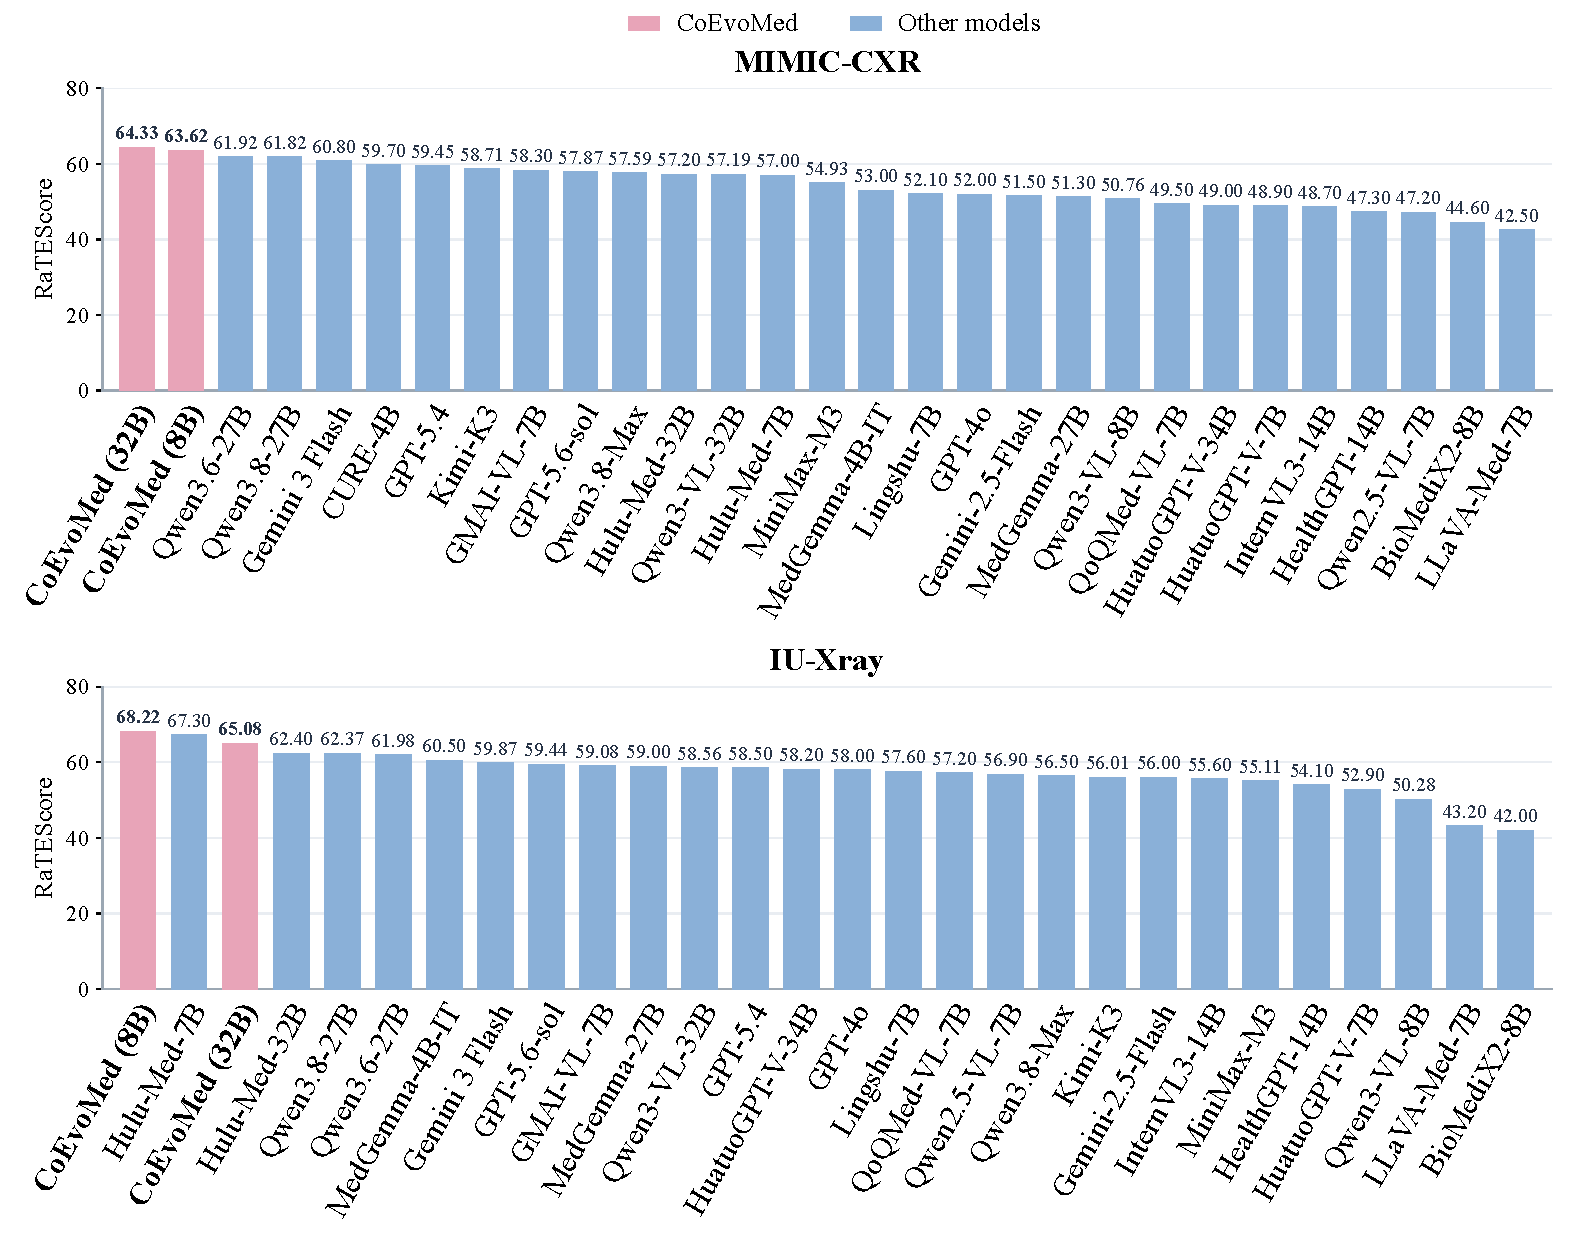
\includegraphics[width=\linewidth,trim=0 14.8bp 0 4bp,clip]{figures/report_ratescore.pdf}
\caption{Report generation on MIMIC-CXR (top, 29 models) and IU-Xray (bottom, 28 models), ranked separately by RaTEScore ($\times100$). Pink denotes CoEvoMed; blue denotes baselines. CURE-4B uses AGRG-29 + GRG. Supplementary metrics appear in Figure~\ref{fig:report_lexical}.}
\label{fig:report_results}
\end{figure}

\paragraph{Applicability to volumetric data.}
CoEvoMed ranks first in the three benchmark summaries in Figure~\ref{fig:3d_main}: M3D-VQA macro accuracy, 3D-RAD macro ROUGE-1, and AMOS-MM RaTEScore. These results extend the evaluation to volumetric question answering and report generation. Category-level results, supplementary metrics, and evaluation details appear in Appendix~\ref{app:3d}.

\begin{figure}[!htb]
\centering
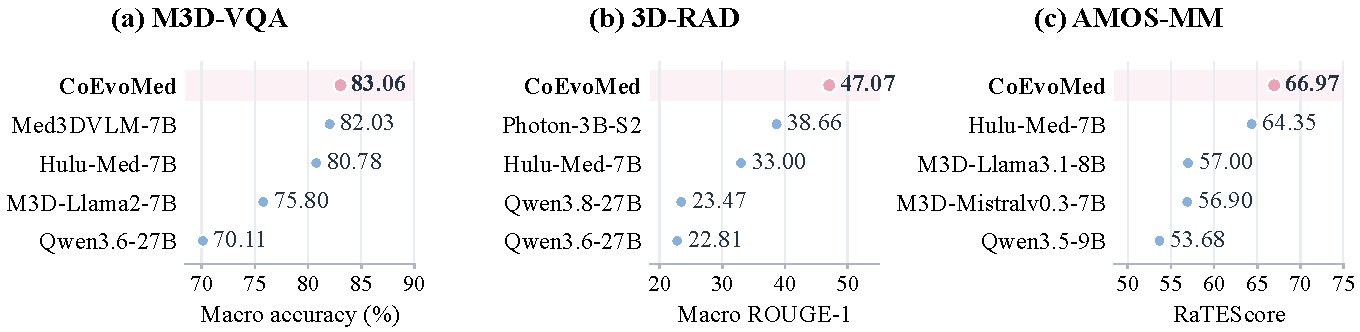
\includegraphics[width=\linewidth]{figures/three_d_main.pdf}
\caption{Volumetric evaluation: (a) M3D-VQA macro accuracy; (b) 3D-RAD macro ROUGE-1; (c) AMOS-MM RaTEScore. Scores are scaled to 100. Each panel shows CoEvoMed (pink) and the four highest-scoring baselines (blue) for its metric within the comparison set in Appendix~\ref{app:3d}.}
\label{fig:3d_main}
\end{figure}

\subsection{Learning dynamics and mechanism analysis}
\label{sec:analysis}
\label{sec:mechanisms}

We examine learning trajectories, feedback--learner alignment, and stage-dependent principle utility. Mechanism comparisons use VQA-RAD and MIMIC-CXR; full results and experimental details appear in Appendix~\ref{app:mechanisms}.

\paragraph{Feedback--learner alignment.}
From the same R5 checkpoint, we jointly vary numerical capability statistics and summaries of error semantics using R2, R3, or R5 validation feedback. Current feedback improves VQA-RAD accuracy by 2.62 percentage points and MIMIC-CXR RaTEScore by 2.77 points, outperforming historical feedback (Table~\ref{tab:ablations}, panel A). This supports aligning curriculum allocation and supervision construction with current capabilities and error patterns.

\paragraph{Dependence on training stage.}
Original and evolved principles show stage-dependent utility at checkpoints after rounds 2 and 5 (R2 and R5) (Table~\ref{tab:ablations}, panel B). On VQA-RAD, original principles lead by 4.22 points at R2, whereas evolved principles lead by 8.26 at R5. On MIMIC-CXR, their difference grows from 0.12 to 9.21 points in favor of evolved principles. This stage dependence supports revising supervision as the learner develops; all six benchmarks appear in Appendix~\ref{app:stage_transfer}.

\begin{table}[H]
\centering\small
\caption{Mechanism ablations: (A) the same R5 learner with R2, R3, or current R5 feedback; (B) original versus evolved construction principles at R2 and R5. VQA-RAD reports accuracy (\%); MIMIC-CXR reports RaTEScore ($\times100$). Reference scores are measured before further training.}
\label{tab:ablations}
\setlength{\tabcolsep}{3.5pt}
\renewcommand{\arraystretch}{1.0}
\begin{minipage}[t]{0.47\linewidth}
\vspace{0pt}
\begin{tabularx}{\linewidth}{Yrr}
\toprule
\multicolumn{3}{l}{\textbf{A. Feedback source at R5}}\\
\midrule
Setting & VQA-RAD & MIMIC-CXR\\
\midrule
R5: Reference & 73.61 & 59.00\\
R2 feedback & 72.51 & 59.11\\
R3 feedback & 71.84 & 58.16\\
\rowcolor{mainOurs} \textbf{R5 feedback} & 76.23 & 61.77\\
\bottomrule
\end{tabularx}
\end{minipage}\hfill
\begin{minipage}[t]{0.50\linewidth}
\vspace{0pt}
\begin{tabularx}{\linewidth}{Yrr}
\toprule
\multicolumn{3}{l}{\textbf{B. Dependence on training stage}}\\
\midrule
Setting & VQA-RAD & MIMIC-CXR\\
\midrule
R2: Reference & 61.64 & 53.31\\
R2: Original & 63.42 & 56.35\\
R2: Evolved & 59.20 & 56.47\\
\midrule
R5: Reference & 73.61 & 59.00\\
R5: Original & 67.97 & 52.56\\
\rowcolor{mainOurs} \textbf{R5: Evolved} & 76.23 & 61.77\\
\bottomrule
\end{tabularx}
\end{minipage}
\end{table}

\paragraph{Cross-backbone applicability.}

On Gemma-3-4B-IT, R7 attains 70.73\% semantic VQA accuracy and 65.89 MIMIC-CXR RaTEScore, improving over Base by 22.39 and 16.23 points (Figure~\ref{fig:gemma_trajectory}). The same checkpoint ties for the highest observed VQA accuracy and achieves the highest report score, supporting applicability beyond Qwen at a smaller model scale. 

\begin{figure}[H]
\centering
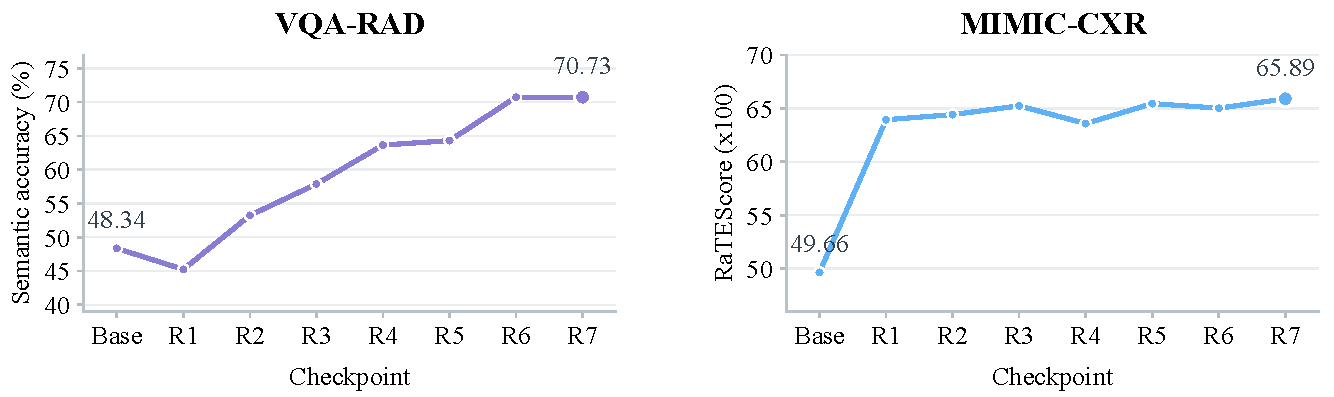
\includegraphics[width=0.85\linewidth]{figures/gemma_trajectory.pdf}
\caption{Cross-backbone evaluation on Gemma-3-4B-IT from Base through R7. VQA-RAD uses semantic accuracy (\%); MIMIC-CXR uses RaTEScore scaled by 100. Both R7 scores belong to the same checkpoint.}
\label{fig:gemma_trajectory}
\end{figure}
\vspace{-10pt}
\begin{figure}[H]
\noindent\begin{minipage}[t]{0.40\textwidth}
\vspace{0pt}
\textbf{Learning trajectories.} Figure~\ref{fig:task_qa} shows that attribute queries improve, organ recognition stabilizes, and localization recovers after declining over R1--R6. These divergent trajectories indicate that capability development is not uniform across tasks, providing the state information used for principle revision and construction allocation. Figure~\ref{fig:trajectory} shows gains on SLAKE, PathVQA, and IU-Xray, peaking at R7--R8. Their agreement with the task-level profiles connects learner responses to externally measured benchmark performance. Together, the profiles characterize capability development and performance on independent external benchmarks.
\end{minipage}\hfill
\begin{minipage}[t]{0.56\textwidth}
\vspace{0pt}\centering
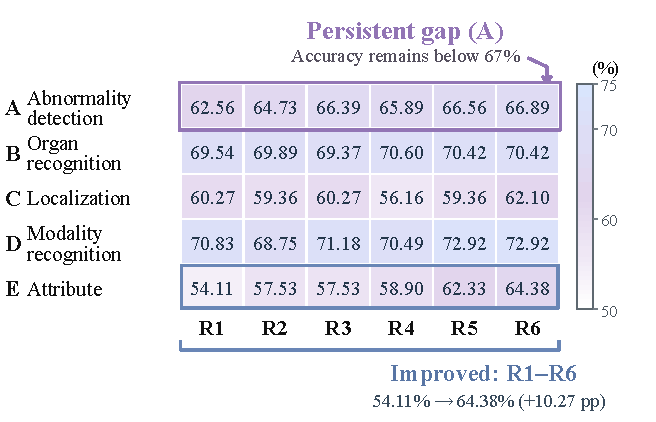
\includegraphics[width=\linewidth]{figures/task_qa_heatmap.pdf}
\caption{Validation accuracy (\%) of the Qwen3-VL-8B learner across five selected QA task categories after completed training rounds R1--R6.}
\label{fig:task_qa}
\end{minipage}
\end{figure}
\vspace{-10pt}
\begin{figure}[H]
\centering
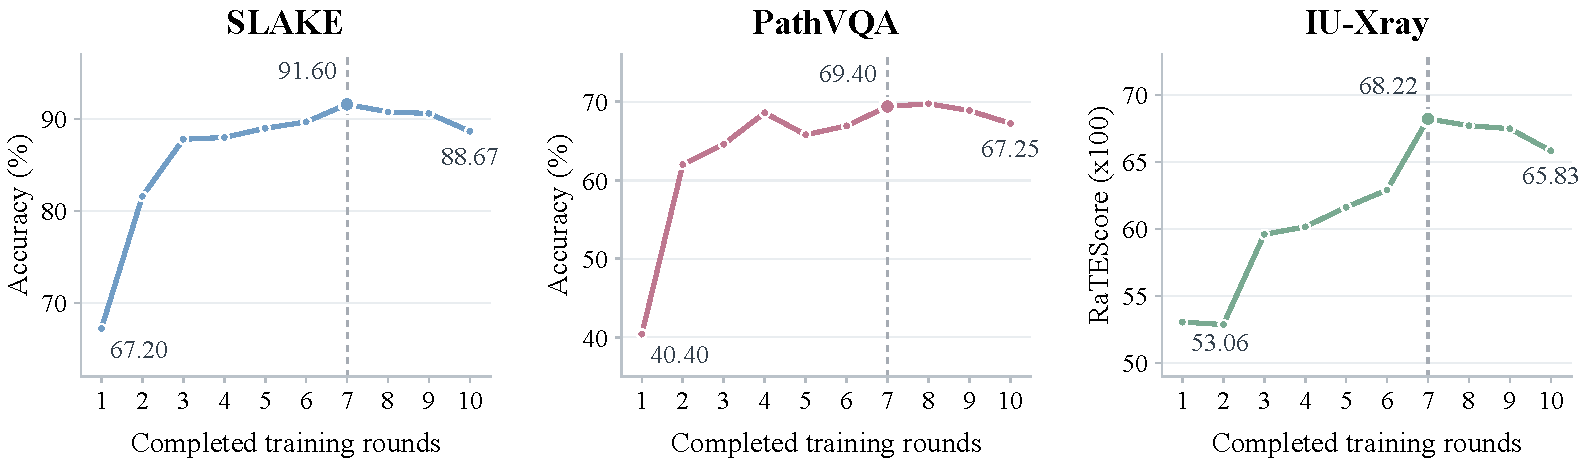
\includegraphics[width=0.85\linewidth]{figures/evolution_trajectory.pdf}
\caption{CoEvoMed-8B trajectories. Dashed lines mark R7, used for all six main 2D results.}
\label{fig:trajectory}
\end{figure}
\vspace{-12pt}
\section{Conclusion}
\label{sec:conclusion}

CoEvoMed treats supervision construction as an evolving component of medical vision--language learning. Construction principles develop in response to the learner's task-specific capabilities, while the resulting supervision shapes subsequent capability development. Curriculum allocation complements this process by distributing a fixed construction budget according to observed learning progress. Multi-agent collaboration connects these two forms of adaptation, using medical evidence to produce supervision whose content and allocation evolve together.

Experiments across 2D VQA, report generation, 3D tasks, and different backbones support the effectiveness of this framework. Comparisons across feedback sources and training stages further show the value of matching supervision construction to the learner's current capability profile. These findings support joint adaptation of how supervision is constructed and where construction effort is allocated as a basis for improving medical multimodal learning.
